\documentclass[11pt, a4paper]{article}

\usepackage{bibentry}
\usepackage[nottoc,numbib]{tocbibind} % References section appears in toc
\usepackage[hidelinks]{hyperref}
\usepackage{graphicx}
\usepackage[margin=1in]{geometry}
\usepackage{url}
\usepackage{booktabs}
\usepackage{amsmath}

\nobibliography*
\setcounter{tocdepth}{2}

\title{A critical review of: Slow rate denial of service attacks against HTTP/2 and detection}
\date{\today}
\author{Bastien DHIVER \\ \href{mailto:bfrd2@kent.ac.uk}{bfrd2@kent.ac.uk}}

\begin{document}
\maketitle
\bibentry{Tripathi:2018}

\tableofcontents
\clearpage

\section{Introduction}

In this paper \cite{Tripathi:2018}, Tripathi and Hubballi seek to assess the security level of the HTTP/2 protocol against Slow Rate Denial-of-Service attacks.
In order to do that, a comparative study with the previous version of the protocol (HTTP/1.1) is conducted.
Five novel attacks against popular HTTP/2 capable web servers are described and their effects measured.
Lastly, a statistical abnormality measurement technique to detect the proposed attacks is discussed and evaluated.

This critical review will evaluate the research conducted by the authors, consider its applicability for a real-life environment and finally, suggest avenues for improvement.

\section{Authors and Institution}

The research was conducted by two Indian researchers, Nikhil Tripathi and Neminath Hubballi.
Both authors carried this research at the Indian Institute of Technology Indore (IIT) in India.
Nikhil is currently a Ph.D. student in the department of Computer Science and is interested in topics such as Computer Networks and Network Security as shown by his publications\footnote{https://scholar.google.co.uk/citations?user=Ur2fiEUAAAAJ}.
One particular area of interest for him is Slow Rate Denial-of-Service attacks.
On the other hand, Neminath is an assistant professor in the department of Computer Science and Engineering and Nikhil's supervisor.
His interests vary from Network security, System Security, Cloud Security and dependable systems. He previously worked for HP, Infosys Lab and Samsung R\&D.

\section{Background}

Background on Denial-of-Service attacks and the HTTP/2 protocol is provided to the reader before getting to the heart of the matter.
Both topics are well introduced.

\subsection{(Distributed) Denial-of-Service attacks}

Four types of attacks are described along their limitations from malicious client's perspective.
Attacks can be performed at both, the transport and the application layer.
A good overview is presented and references are given while doing so.
This is a good choice to present attacks at various layers as the most commonly seen are the Transport-level DDoS Flooding attacks.
We can get an idea of the proportions as shown from a recent Akamai report \footnote{https://www.akamai.com/us/en/multimedia/documents/state-of-the-internet/q4-2017-state-of-the-internet-security-report.pdf} on Figure \ref{fig:akamai}.
\begin{figure}[ht]
	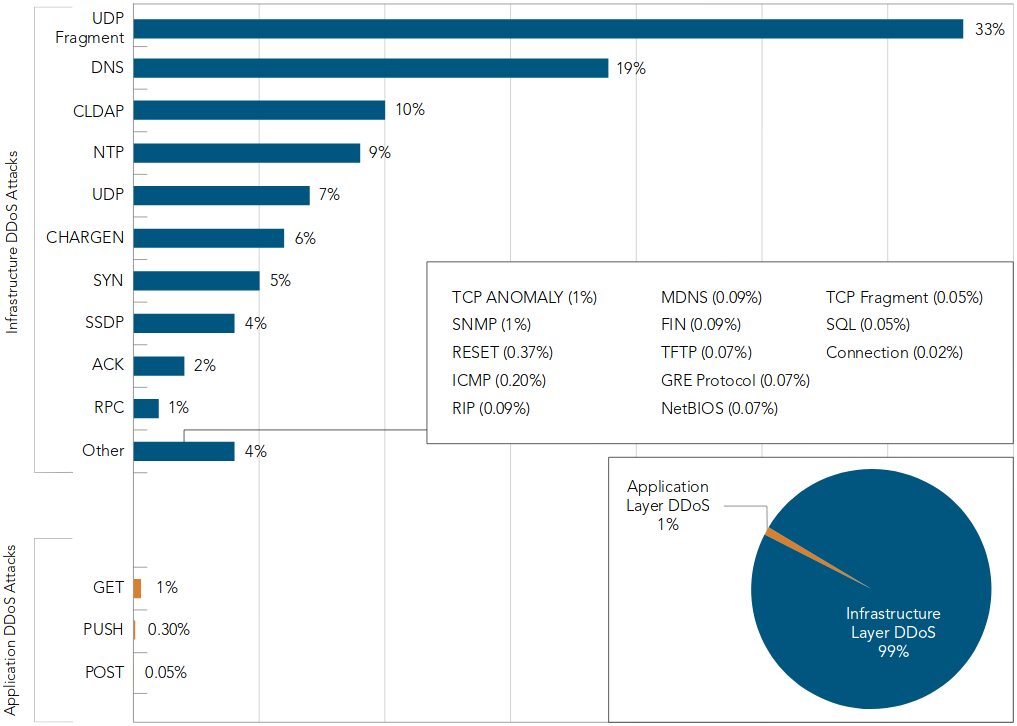
\includegraphics[scale=0.40]{images/akamai2017DDoSAttackVectorFrequency.png}
	\caption{DDoS Attack Vector Frequency, Q4 2017 from Akamai}
	\label{fig:akamai}
\end{figure}
They succeed to pinpoint the drawbacks of non-slow rate attacks which are their easy detection and the resources needed for an attacker to perform such attacks (network bandwidth, computational resources).
They chose to target the number of available slot in web servers connection queue which is smart because their limited number make them more vulnerable and the effects, really powerfull.
In this process, looking as much as possible as legitimate traffic is the key to avoid detection.
DoS attacks frequency is growing as well as their intensity and the associated costs as report Neustar\cite{Neustar:report}.
The threat is real, the financial impacts costly in addition to the loss of customers and the image of the company damaged.

\subsection{HTTP/2}

The HTTP/2 protocol is quickly introduced with a description of essentials frames along a diagram representing an exchange during a basic transaction.
This helps the reader to quickly get an overview of how the protocol works.
The cleartext version of HTTP/2 (h2c) is not used by web browsers though, TLS is a De Facto standard, even if it wasn't included in the standard\footnote{https://http2.github.io/faq/\#does-http2-require-encryption}.
With that in mind, the exchanges between a server and a client are different, as shown by this Wireshark network capture I made on Figure \ref{fig:wireshark}. The decryption process is described in this presentation\footnote{https://sharkfesteurope.wireshark.org/assets/presentations17eu/15.pdf}.
\begin{figure}[ht]
	\centering
	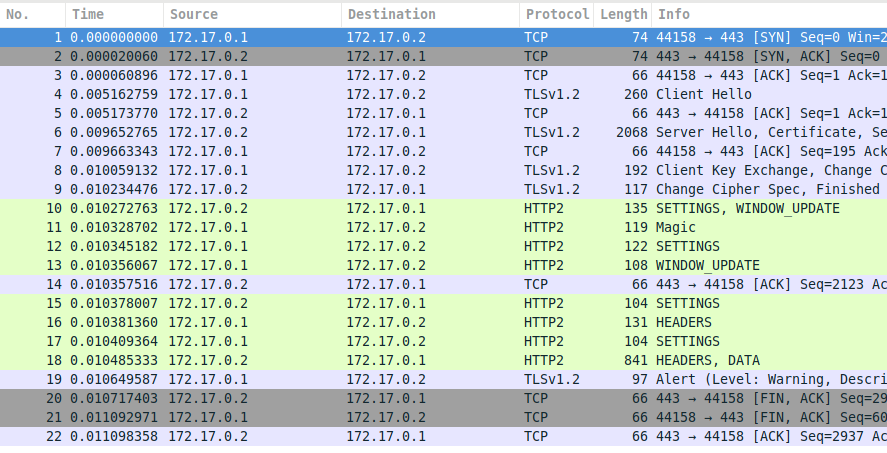
\includegraphics[scale=0.5]{images/HTTP2BasicExchangeNginxCurl.png}
	\caption{Decrypted HTTP/2 exchange between Nginx and curl displayed in Wireshark, client IP address is 172.17.0.\textbf{1}}
	\label{fig:wireshark}
\end{figure}
We can see that after the TCP and the TLS handshakes, the server is the one to send the first frames.
Taking that into account and updating the diagram could have been a good idea here.

\section{Reviewing main points of the article}

A review of three important parts will be made, considering the testbed set up, the proposed attacks and their detection.

\subsection{Testbed}

The authors selected four popular web servers that supports the HTTP/2 protocol, namely Apache, Nginx, H2O and Nghttp2.
The web servers were installed on a penetration testing GNU/Linux distribution named Kali.
This doesn't reflect environments used in production but since this distribution is based on Debian, it's not an issue.
At the time of this writing, the Debian distribution is used by 30\% of the websites hosted on a GNU/Linux system\footnote{https://w3techs.com/technologies/details/os-linux/all/all}, just behind Ubuntu with it's 37\%, which is based on Debian as well.
The Proofs-of-Concept attacks were implemented in Python by the authors which makes sense since it's commonly used to demonstrate and validate such assumptions.
A well-known benchmarking tool named h2load was used to create and sent legitimate traffic.
The architecture set up is very simple but sufficient to test and measure the attacks effects.
Monitoring could have been put in place to provide graphs of the target resources usage.

\subsection{The attacks}

Five novel and effective attacks targeting the number of free connection slots available of popular web servers are described by the authors along with the measured effects.
Clear interaction diagrams at protocol level are provided for every attack and it really helps to understand how they are conducted and how they can be implemented.
All of them requires a single HTTP payload with no more than four frames in order to cause the desired effects.
This confirms the low level of interaction required to perform slow rate DoS.
In the majority of cases, they require the client to re-send the payload after a specific timeout as the connections are closed by the server.
We can consider them as novel because no mentions of such attacks on HTTP/2 were found so far in the literature.

\subsubsection{Effects}

The measured effects put Apache as the more vulnerable of the four tested servers.
Their results claimed that only 150 connections were able to create a DoS scenario no matter which attack is performed on this web server.
It also put in perspective that some servers had infinite timeout values depending on the attacks except for the web server Nghttp2.
The paper does not focus on CPU, RAM, network usage and processes states of the targeted system, it could have strengthened the stealth claims that were made.
An observation I had is that the behaviour of web servers are different in terms of timeout values and frames sent back, this can easily lead to software fingerprinting.
The authors tested the attacks effects over TLSv1.2 as well which is realistic.
Even if TLSv1.3 has just been approved by the IETF two weeks ago\footnote{https://www.ietf.org/mail-archive/web/ietf-announce/current/msg17592.html}, TLSv1.2 is and will stay the default for a little while.
Researchers used the Python Scapy packet manipulation program to perform the TLS handshake and then sent hardcoded payloads.
It would have been so much easier to wrap the TLS context over the TCP socket to avoid the overhead mentioned.
A comparison of slow rate DoS attacks in HTTP/1.1 and HTTP/2 is made with the Apache web server and focuses on structurally similar attacks such as Slow read, Slow message body and slow header.
The slow message body and slow header are effective in both cases but the slow read attack is only effective on HTTP/2.

\subsection{Detection}

Current web traffic is collected during the testing phase and then compared with the legitimate traffic previously collected from the training phase.
A set of five features closely linked to the protocol is defined.
A distance measurement technique using chi-square test statistics is used to measure the deviation between the recorded phases.
The authors developed a program to extract the required features but no code was provided\ldots~
Their program uses a Java library, why not use the Python Scapy library they mentioned page 9?
This library is well suited for packet manipulation and inspection.
One claimed contribution of the authors on page 2 is:
\begin{quote}
	We also propose a novel detection mechanism to detect these Slow Rate DoS attacks.
\end{quote}
Well, the usage of the chi-square method for detecting anomalies in network traffic with profiles and feature selection isn't new at all \cite{Feinstein:2003} and has been used since 2003 at least.

\subsubsection{Setup}

A sample website has been put in place, with images and an upload form to perform their tests.
Few volunteering users were asked to access the sample website.
The setup seams credible enough.
Apache was chosen to perform the tests which isn't a bad choice regarding its adoption over the web\footnote{https://news.netcraft.com/archives/2018/02/13/february-2018-web-server-survey.html} as shown by Figure \ref{fig:netcraft}.

\begin{figure}[ht]
	\centering
	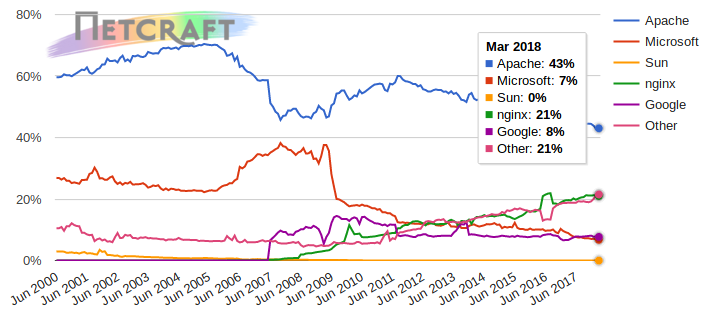
\includegraphics[scale=0.5]{images/netcraftWebServersUsage.png}
	\caption{\href{https://news.netcraft.com/archives/2018/02/13/february-2018-web-server-survey.html}{Percentages of websites using various web servers by Netcraft}}
	\label{fig:netcraft}
\end{figure}
It's also worth noting that the proposed technique used for detection with encrypted HTTP/2 traffic which uses intercepting proxy could not work out of the box depending on software implementations due to the deployment of TLSv1.3\footnote{https://www.imperialviolet.org/2018/03/10/tls13.html}.

\subsubsection{Detection Performance}

Recall and False Positive Rate are used as performance metrics and graphs are provided.
The detection scheme will have a high accuracy detection only if the connection pool space is consumed for a definite amount of time.
The sending rate is so slow that the measured traffic profile is almost similar to normal HTTP/2 traffic.
The detection performance depends on the threshold chosen for $\chi^2$ value and the size of the window period (\Delta T) chosen for monitoring features.
Since the attacks mimic real traffic, this threshold will eventually be set to a lower value which can lead to a false positive increase.
The overall effects look a bit mixed unfortunately.

\section{Prior work}

Authors are well aware of the relation of their work with existing literature.

\subsection{Vulnerabilities in HTTP/2 protocol}

I only could find two papers by Adi and al.~\cite{Adi:2015}\cite{Adi:2016}, a Ph.D. thesis \cite{Adi:2017} and a report by Imperva~\cite{Imperva:h2} that discussed DoS attacks against HTTP/2.
The researchers found the same resources.
The thesis was not available at the time their research was published.
A comparison of the proposed attacks with the attacks discussed in Adi et al. is provided.
A small mistake is made, they confused the number of packets with the number of connections required.
Tripathi and Hubballi give credibility of their attacks compared to the described ones since the latter are based on flooding which makes the detection trivial and the impact is a reduction of Quality (RoQ) only.
The two other resources mentioned mainly reported implementation issues that have been patched since.

\subsection{Anomalies in encrypted network traffic}

Observing properties such as inter-packet arrival time and time gaps between a request and its corresponding response can be used to detect anomalies in encrypted network traffic.
Why didn't the authors explore the subject a little more?
No intercepting proxy is needed and it could be sufficient to detect the proposed attacks.

\subsection{Chi-square test}

Chi-square test is widely used to detect network intrusions, port scanning and botnet control servers (C2) among others with a decent accuracy.
This is the only detection test mentioned in the paper, more literature review could have help to mention a couple of alternatives such as machine learning techniques.

\section{Applicability of Research}

The paper is fairly recent, it has been submitted in 2017, published in 2018 and referenced on ACM\footnote{https://dl.acm.org/citation.cfm?id=3162826}.
HTTP/2 deployment and adoption is growing to reach nearly 25\% as shown by Figure \ref{fig:h2adopt}.
\begin{figure}[ht]
	\centering
	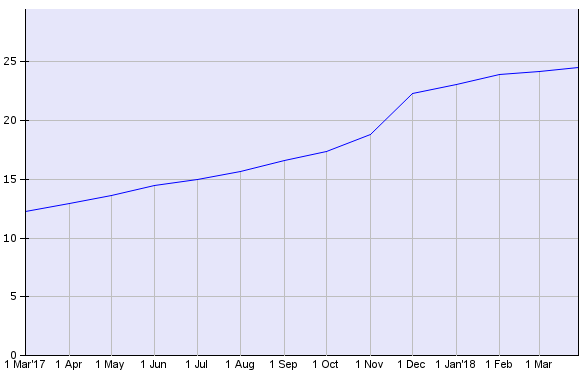
\includegraphics[scale=0.6]{images/http2WebsitesUsage.png}
	\caption{\href{https://w3techs.com/technologies/details/ce-http2/all/all}{Usage of HTTP/2 for websites by W3Techs.com (29 Mar 2018)}}
	\label{fig:h2adopt}
\end{figure}
This is a timely subject and not a week/month goes by without hearing about DoS attacks and their growing impacts.
Authors used real web servers that are widely used all over the Internet, setup credible testbeds and demonstrated the real effects of the proposed attacks.
This research can be the basis of building detection mechanisms for real world production environments once plugins for web servers and/or proxies will appear.

\section{Criticisms}

\subsection{Proof-of-Concept}

The authors claimed to have implemented the attacks in Python, but no links or references to the code are provided whatsoever.
I had to implement them to verify the veracity of the claimed effects.
The code is published on my GitHub account\footnote{https://github.com/Dhiver/SlowRate-HTTP2-DoS}.
I conducted tests with the Apache 2.4.23 and Nghttp2 1.14.0 with the same setup as the authors.
The software have been fetched from the original websites and compiled in an isolated environment.
I noted several differences with the authors' results as shown by Table \ref{tab:results}.

\begin{table}[ht]
\begin{tabular}{@{} lr c c c c c c @{}}
	\toprule
		Server & Attack 1 & Attack 2 & Attack 3 & Attack 4 & Attack 5 & \textnumero~conn\\
	\midrule
		Apache & 60 & 120 & 60 & 60 & 5 & 400\\
		Nghttp2 & 10 & 10 & 10 & 10 & 10 & >3000\\
	\bottomrule
\end{tabular}
	\centering
    \caption{Connection waiting time in seconds and \textnumero~at servers for the five attacks}
	\label{tab:results}
\end{table}

The waiting time values are less spectacular than the announced ones as well as the number of connections required to feel the whole queue unfortunately.

\subsection{Erwin Adi Ph.D. Thesis}

	\begin{quote}
		"Denial-of-service attack modelling and detection for HTTP/2 services"
	\end{quote}

The thesis \cite{Adi:2017} lists four novel flood attacks against HTTP/2.
Four machine learning techniques to conduct traffic analysis that has been proven suitable for detection are used (Naïve Bayes, Decision Tree, JRip and Support Vector Machines).
Flash-crowded traffic is used to populate the dataset of legitimate network traffic.
Different features less specific to HTTP/2 protocol were used such as the number of connections and the flow information.
However, the mentioned attacks require a high number of packets and are a more prone to detection as they are based on flooding attacks.
Machine learning techniques had high accuracy in classifying network traffic thus making them suitable to detect DoS attacks.
Detection is not only based on protocol specific features, other properties are useful such as, the entropy of requests per source IP addresses, the traffic flow (number of packets, their size, \ldots), the behaviour of hosts and the statistics on the traffic.
The same detection performance metrics are used here, the recall and FPR rates.
The attacks described by Tripathi and Hubballi are much more subtle than what's described by Adi.

\subsection{Personnal opinion}

Here is my opinion in addition to the comments I have left throughout the sections.
Tripathi and Hubballi demonstrated that a single client can create a DoS of widely used HTTP/2 web servers.
Their selection of web servers is a good one.
The paper is effortless to read, of good quality and very specific to HTTP/2.
It was a good idea to focus on the number of available slot connection.
However, where are the Proofs-of-Concept??
The PoC of the attacks, the feature extraction code and the detection system code are missing.
I had to implement the attacks in order to verify the claims\ldots~
How do you expect to be credible of you don't provide concrete proofs?
The cleartext version of HTTP/2 is used to describe the interactions but it differs from a real-life environment.
When I first read the paper the attacks seemed quite simple and spectacular, but after running my tests I was a bit disappointed.
Nevertheless, good job!

\section{Avenues for Improvement}

In addition to the comments I made in the upper sections, I will mention a few more areas for improvement.
Only the chi-square statistical test is mentioned.
Today everything is about machine learning, we want to read about machine learning techniques!
A Future Works section could have been a good opportunity to talk about the release of a web server detection module for example.
No countermeasures were provided at all.
We would have liked to see advices such as the configuration of various timeouts in web servers to mitigate the effects in some extents.
We also wonder if the discoveries have been reported to the software companies.

\section{Conclusion}

New layer seven attacks were described in this research.
I was interested in learning more about the HTTP/2 protocol and had little knowledge about Slow Rate DoS attacks.
This reading awakened my curiosity on both subjects.
An overall view is that the HTTP/2 protocol security assessment is still in its very preliminary stages.
We are hoping to see more studies in the next couple of months!

%% --- References

\bibliography{refs}
\bibliographystyle{unsrt}

\end{document}
